\chapter{YSO}

\begin{table}[h]
  \begin{center}
    \caption{Y$_{2}$SiO$_{5}$ theoretical second-order elastic coefficients (GPa)}
    \label{tab:elasticcoefficients}
    \begin{tabular}{l|r r r r r r r r r r r r r r} 
    \hline % <-- Changed to S here.
Space group & $c_{11}$ & $c_{22}$ & $c_{33}$ & $c_{44}$ & $c_{55}$ & $c_{66}$ & $c_{12}$ & $c_{13}$ & $c_{15}$ & $c_{23}$ & $c_{25}$ & $c_{35}$ & $c_{46}$ \\
       \hline
$B2/b$~\citep{doi:10.1111/jace.12764} & 226 & 201 & 156 & 44 & 67 & 63 & 88 & 59 & 5 & 27 & -0.3 & -0.2 & 10 \\ 
$C2/c$~\citep{Ceramics} & 226 & 156 & 201 & 44 & 63 & 67 & 59 & 88 & 5 & 27 & -0.3 & -0.2 & 10 \\
\hline
    \end{tabular}
  \end{center}
\end{table}

\begin{table}[h]
  \begin{center}
    \caption{Y$_{2}$SiO$_{5}$ theoretical second-order elastic coefficients}
    \label{tab:elasticcoefficients}
    \begin{tabular}{l|r r r r r r r r r r r r r r} 
    \hline % <-- Changed to S here.
Space group & $c_{11}$ & $c_{22}$ & $c_{33}$ & $c_{44}$ & $c_{55}$ & $c_{66}$ & $c_{12}$ & $c_{13}$ & $c_{15}$ & $c_{23}$ & $c_{25}$ & $c_{35}$ & $c_{46}$ \\
       \hline
$C2/c$ & 226 & 156 & 201 & 44 & 63 & 67 & 59 & 88 & 5 & 27 & -0.3 & -0.2 & 10 \\
\hline
    \end{tabular}
  \end{center}
\end{table}





\begin{figure}[H]
    \centering
    \begin{subfigure}[b]{0.487\textwidth}
        \centering
        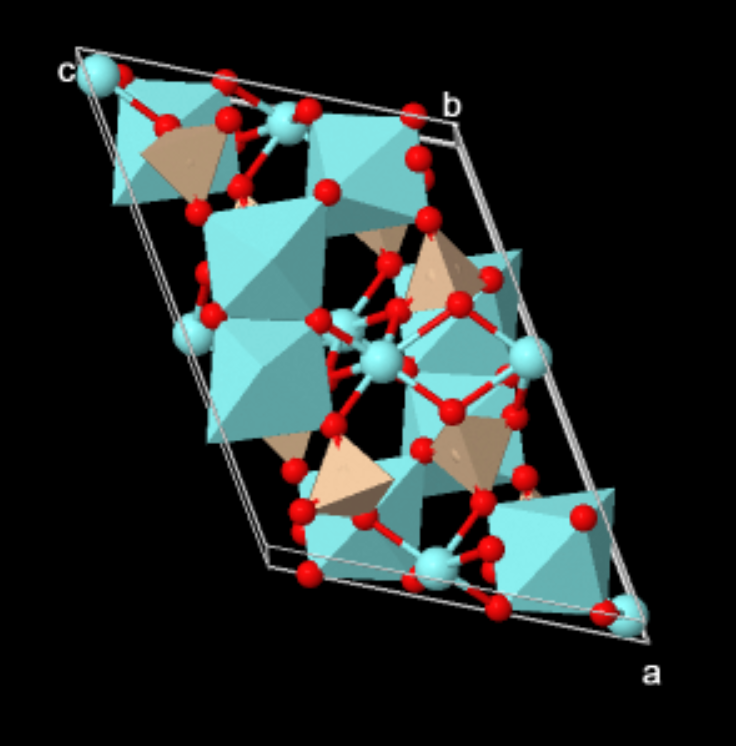
\includegraphics[width=\textwidth]{C2c}
        \caption{$C2/c$}
    \end{subfigure}
%     \hfill
    \begin{subfigure}[b]{0.4\textwidth}
        \centering
        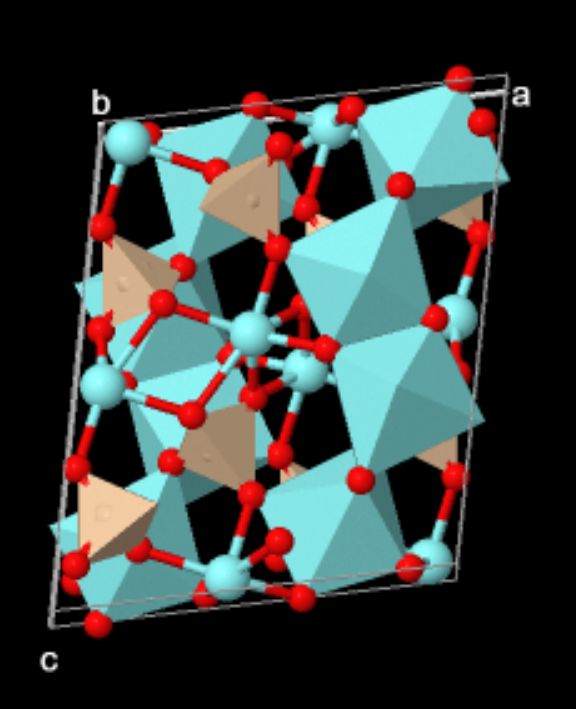
\includegraphics[width=\textwidth]{I2a}
   \caption{$I2/a$}
   \end{subfigure}
    \caption{Comparison of the Y$_{2}$SiO$_{5}$ unit cell for the (a) $C2/c$ and (b) $I2/a$ space group obtained from the inorganic crystal structure database (collection code: 291362).}
\label{fig:crystalspacegroups}
\end{figure}

\begin{table}[h]
 \begin{center}
  \caption{Y$_{2}$SiO$_{5}$ $I2/a$ lattice parameters\citep{doi:10.1021/acsami.5b00445}.}
  \label{tab:I2alatticeparam}
  \begin{tabular}{l | c}
  \hline
  Lattice constants & Theoretical\\
  \hline
  a ($\AA$) &  10.40\\
  b ($\AA$) &  6.71\\
  c ($\AA$) &  12.47\\
  $\beta$ ($^{\circ}$) &  102.6\\
  \hline
    \end{tabular}
  \end{center}
\end{table}

\begin{figure}[h]
\centering
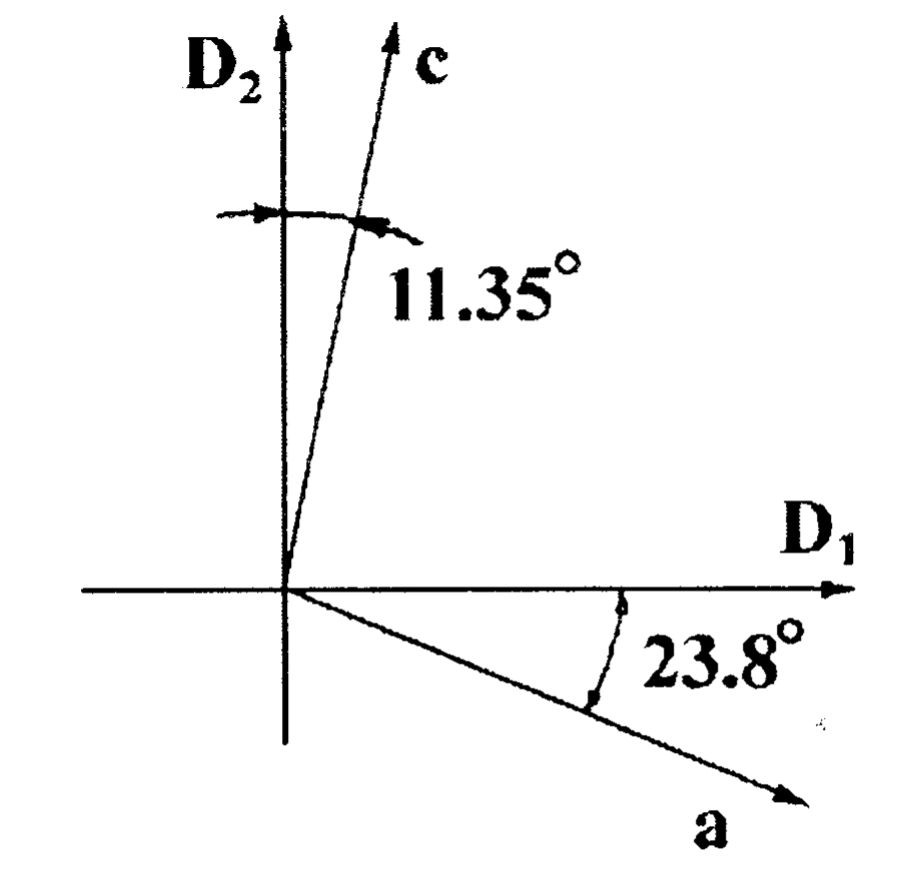
\includegraphics[height=0.32\textwidth,keepaspectratio]{D1bD2abc}
\caption{\label{fig:D1bD2abc} Orientation of YSO $C2/c$ crystallographic axis with respect to the optical axis \citep{SHOUDU1999901}.}
\end{figure}




